\section{Experimental Setup}
\label{sec:Evaluation}
This section presents the details of our experimental study such as benchmark datasets, experimental design, and evaluation measures.
%In RQ1, we validate
% prediction models built by defect datasets. In addition, we were interested
% in verifying if our framework can build prediction models from non-defect
% datasets. Thus, in RQ2, we check prediction performance of models built by
% different types of non-defect datasets: software engineering (SE) and non-SE datasets.
% We conducted experiments using 28 defect datasets in 5 groups with different
% metric sets.


% The RQ3 is to verify whether our cross-domain prediction models can conduct
% cross-prediction for all target projects. Prediction coverage~\sung{Should we mention this in the approach? If we don't have any matching features based on your threshold, we cannot predict? Then, say, we investigate this in experiments.} represents how
% many target projects could be predicted by using our cross-domain models. If
% there are no feasible~\sung{Need to explain in detail in Approach.} prediction combinations for a certain target project, it
% might be difficult to use a cross-domain prediction model in practice.
%In previous studies on cross-project defect prediction,
%feasibility rate of cross prediction combinations were quite low (about
%3-5\%)~\cite{He12,Zimmermann09}.
% Thus, we address RQ3 by measuring prediction coverage.
\subsection{Benchmark Datasets}

\begin{table}[t]
%\scriptsize
\centering
\caption{The 34 defect datasets from five groups.}
\label{tab:datasets}
%\setlength{\tabcolsep}{5pt}
%\setlength{\extrarowheight}{1.5pt}
\begin{tabular}{|@{}c@{}|@{}c@{}|c|c|@{}c@{}|@{}c@{}|}
\hline
	\multirow{2}{*}{\textbf{Group}}
	&\multirow{2}{*}{\textbf{Dataset}}
	&\multicolumn{2}{c|}{\textbf{\# of instances}}
	&\multirow{2}{*}{\textbf{\specialcell{\# of\\metrics}}}
	&\multirow{2}{*}{\textbf{\specialcell{Prediction \\ Granularity}}}
	\\ \cline{3-4}
	
	&
	&\textbf{All}
	&\textbf{Buggy(\%)}
	&
	&
	\\ \hline \hline
\multirow{5}{*}{\specialcell{AEEEM~\\\cite{DAmbros12,Nam13}}}
	&	EQ
	&\centering324
	&	129 (39.81\%)
	& \multirow{5}{*}{61}
	& \multirow{5}{*}{Class}
	\\ %\cline{4-5}

	&	JDT
	&\centering997
	& 206 (20.66\%)
	& &
	\\ 

	&	LC	
	&\centering691
	& 64 (9.26\%)
	& &
	\\ 
	
	&	ML	
	&\centering1862
	& 245 (13.16\%)
	& &
	\\ 
	
	&	PDE
	&\centering1492
	& 209 (14.01\%)
	& &
	\\ \hline
	
\multirow{3}{*}{\specialcell{ReLink\\\cite{Wu11}}}
	&	Apache
	&\centering194
	&	98 (50.52\%)
	& \multirow{3}{*}{26}
	& \multirow{3}{*}{File}
	\\ %\cline{4-5}

	&	Safe
	&\centering56
	& 22 (39.29\%)
	& &
	\\ 
	
	&	ZXing
	&\centering399
	& 118 (29.57\%)
	& &
	\\ \hline
% \multirow{3}{*}{MIM~\cite{Lee11}}
% 	&	MIMEtc
% 	&\centering1042
% 	&	57(5.40\%)
% 	& \multirow{3}{*}{113}
% 	\\ %\cline{4-5}
% 
% 	&	MIMMylyn
% 	&\centering1061
% 	& 152(14.30\%)
% 	& 
% 	\\ 
% 	
% 	&	MIMTeam
% 	&\centering239
% 	& 85(35.50\%)
% 	& 
% 	\\ \hline
	
\multirow{10}{*}{\specialcell{MORPH\\\cite{Peters12}}}
	&	ant-1.3
	&\centering125
	&	20 (16.00\%)
	& \multirow{10}{*}{20}
	& \multirow{10}{*}{Class}
	\\ %\cline{4-5}

	&	arc
	&\centering234
	& 27 (11.54\%)
	& &
	\\ 
	
	&	camel-1.0
	&\centering339
	& 13 (3.83\%)
	& &
	\\
	
	&	poi-1.5
	&\centering237
	& 141 (59.49\%)
	& &
	\\ 
	
	&	redaktor
	&\centering176
	& 27 (15.34\%)
	& &
	\\ 
	
	&	skarbonka
	&\centering45
	& 9 (20.00\%)
	& & 
	\\ 
	
	&	tomcat
	&\centering858
	& 77 (8.97\%)
	& &
	\\ 
	
	&	velocity-1.4
	&\centering196
	& 147 (75.00\%)
	& &
	\\ 
	
	&	xalan-2.4
	&\centering723
	& 110 (15.21\%)
	& &
	\\ 
	
	&	xerces-1.2
	&\centering440
	& 71 (16.14\%)
	& &
	\\ \hline

\multirow{11}{*}{\specialcell{NASA\\\cite{promise12,Shepperd13}}}
	&	cm1
	&\centering344
	&	42 (12.21\%)
	& \multirow{5}{*}{37}
	& \multirow{11}{*}{Function}
	\\ %\cline{4-5}

	&	mw1
	&\centering264
	& 27 (10.23\%)
	& &
	\\

	&	pc1
	&\centering759
	& 61 (8.04\%)
	& &
	\\

	&	pc3
	&\centering1125
	& 140 (12.44\%)
	& &
	\\

	&	pc4
	&\centering1399
	& 178 (12.72\%)
	& &
	\\ \cline{2-5}

	&	jm1
	&\centering9593
	& 1759 (18.34\%)
	& 21 &
	\\ \cline{2-5}

	&	pc2
	&\centering1585
	& 16 (1.01\%)
	& 36 &
	\\ \cline{2-5}

	&	pc5
	&\centering17001
	& 503 (2.96\%)
	& 38 &
	\\ 

	&	mc1
	&\centering9277
	& 68 (0.73\%)
	& 38 &
	\\ \cline{2-5}

	&	mc2
	&\centering127
	& 44 (34.65\%)
	& 39 &
	\\

	&	kc3
	&\centering200
	& 36 (18.00\%)
	& 39 &
	\\ \hline
	
\multirow{5}{*}{\specialcell{SOFTLAB\\\cite{Turhan09}}}
	&	ar1
	&\centering121
	&	9 (7.44\%)
	& \multirow{5}{*}{29}
	& \multirow{5}{*}{\specialcell{Function}}
	\\ %\cline{4-5}

	&	ar3
	&\centering63
	& 8 (12.70\%)
	& &
	\\ 

	&	ar4
	&\centering107
	& 20 (18.69\%)
	& &
	\\ 
	
	&	ar5	
	&\centering36
	& 8 (22.22\%)
	& &
	\\ 
	
	&	ar6
	&\centering101
	& 15 (14.85\%)
	& &
	\\ \hline	

\end{tabular}
\end{table}

We collected publicly available datasets from previous
studies~\cite{DAmbros12,Nam13,Peters12,Turhan09,Wu11}.
Table~\ref{tab:datasets} lists all dataset groups used in our experiments. Each
dataset group has a heterogeneous metric set as shown in the table.
Prediction Granularity in the last column of the table means the prediction
granularity of instances. Since we focus on the distribution or correlation of
metric values when matching metrics, it is beneficial to be able to
apply the HDP approach on datasets even in different granularity levels.
% Table~\ref{tab:SE_datasets} and~\ref{tab:non-SE_datasets} list
% non-defect (SE and non-SE) datasets, which were used only for training
% prediction models in our study.

% \begin{figure}[t]
% 	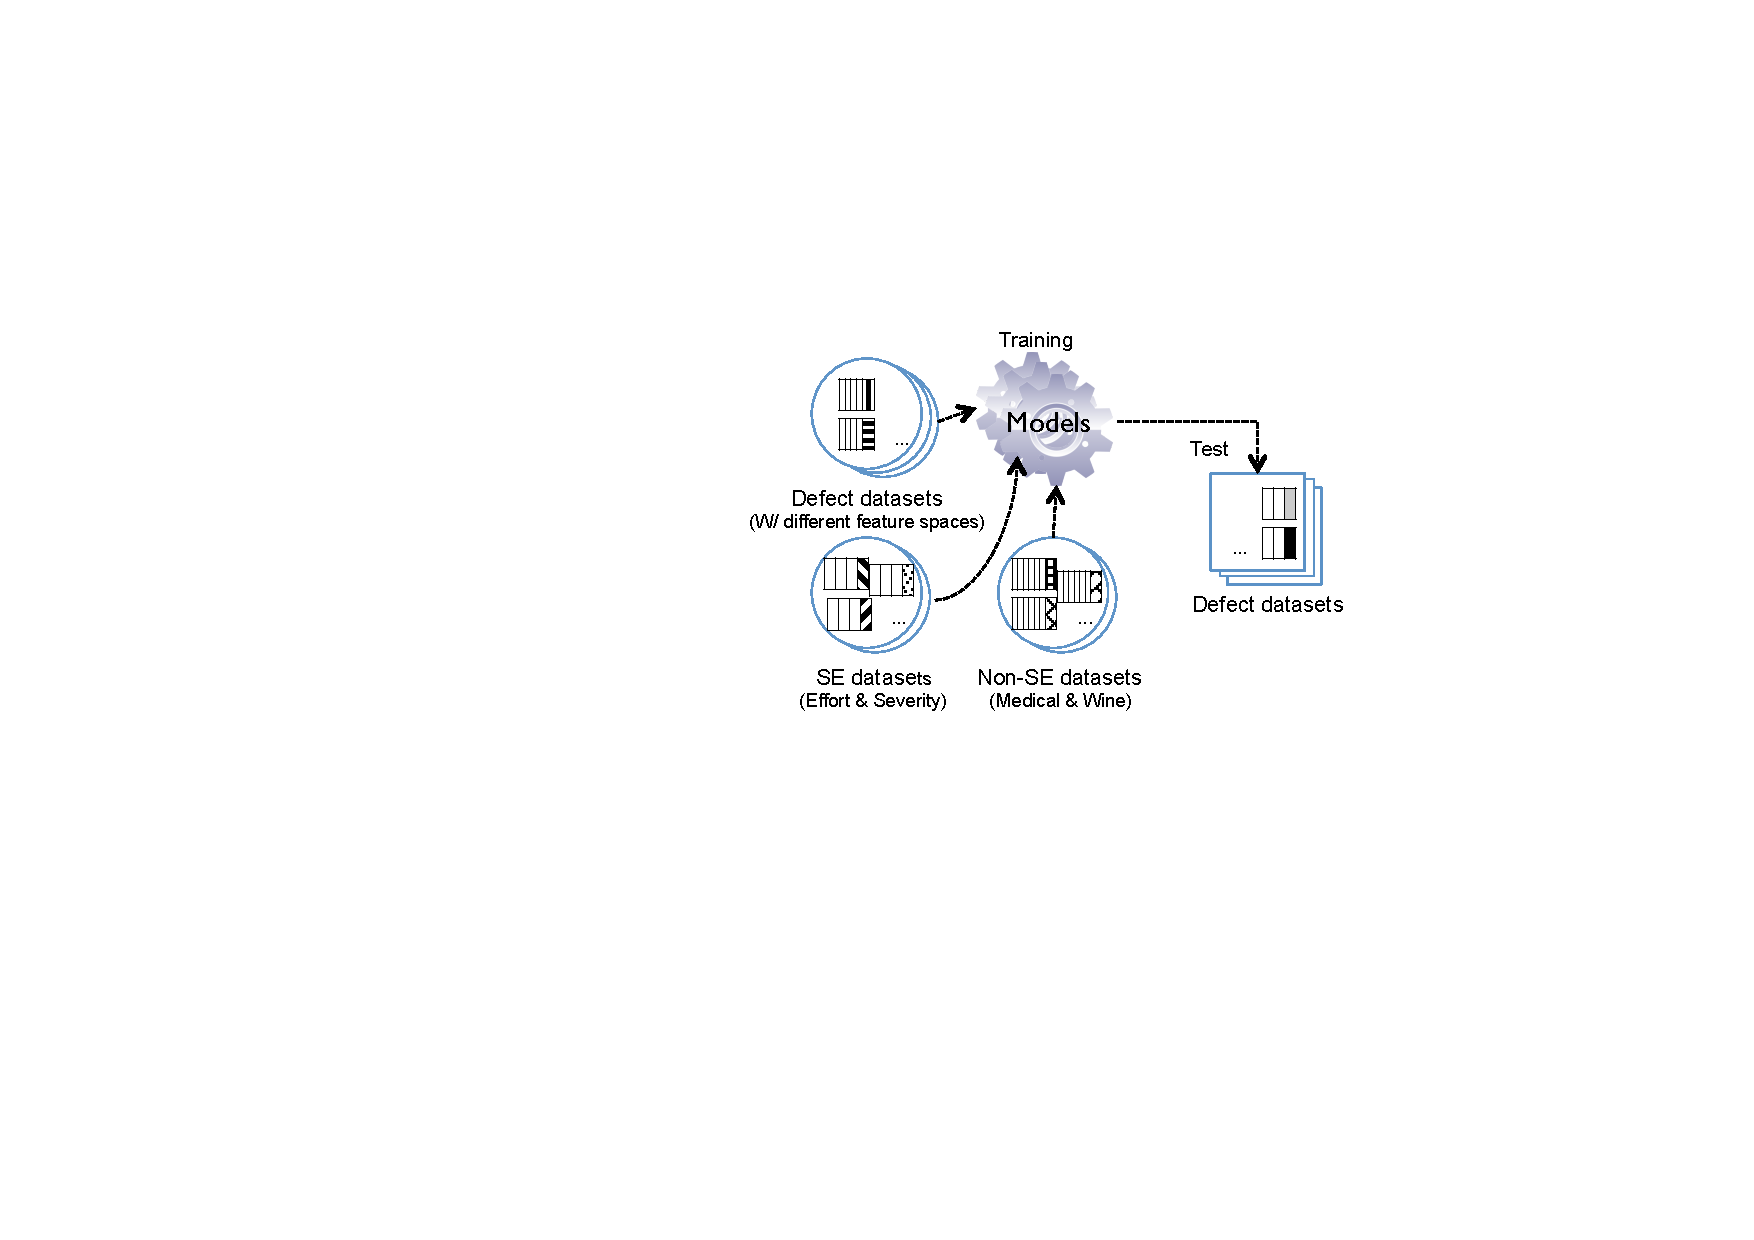
\includegraphics[width=\linewidth]{Figures/overview.pdf}
% 	\caption{Overview of cross-domain defect prediction across benchmark datasets.}
% 	\label{fig:overview}
% \end{figure}
% 
% Figure~\ref{fig:overview} describes the overview of our cross-domain defect
% prediction across benchmark datasets. We validated our framework using
% models built by defect, SE, or non-SE for testing defect datasets.

We used five groups with 34 defect datasets: AEEEM, ReLink, MORPH, NASA,
and SOFTLAB.

AEEEM was used to benchmark different defect
prediction models~\cite{DAmbros12} and to evaluate CPDP
techniques~\cite{He14,Nam13}.
Each AEEEM dataset consists of 61 metrics including object-oriented (OO) metrics,
previous-defect metrics, entropy metrics of change and code, and churn-of-source-code
metrics~\cite{DAmbros12}.

Datasets in ReLink were used by Wu et
al.~\cite{Wu11} to improve the defect prediction performance by increasing the quality of the
defect data and have 26 code complexity metrics extracted by the Understand
tool~\cite{Understand}.

The MORPH group contains defect datasets of several open source projects used in
the study about the dataset privacy issue for defect prediction~\cite{Peters12}.
The 20 metrics used in MORPH are McCabe's cyclomatic metrics, CK metrics, and
other OO metrics~\cite{Peters12}.

NASA and SOFTLAB contain proprietary
datasets from NASA and a Turkish software company, respectively~\cite{Turhan09}.
We used 11 NASA datasets in the PROMISE
repository~\cite{promise12,Shepperd13}. Some NASA datasets have different metric sets as shown in Table~\ref{tab:datasets}. We used cleaned NASA datasets (DS$'$ version)~\cite{Shepperd13}.
For the SOFTLAB group, we used all SOFTLAB datasets in the PROMISE
repository~\cite{promise12}. The metrics used in both NASA and SOFTLAB groups
are Halstead and McCabe's cyclomatic metrics but NASA has additional
 complexity metrics such as {\em parameter count} and {\em percentage of comments}~\cite{promise12}.

Predicting defects is conducted across different dataset
groups.
For example, we build a prediction model by Apache in ReLink and tested the
model on velocity-1.4 in MORPH
(Apache$\Rightarrow$velocity-1.4).\footnote{Hereafter a rightward arrow
($\Rightarrow$) denotes a prediction combination.} Since some NASA datasets do not have the same metric sets, we also conducted cross prediction between some NASA datasets that have different metric sets, e.g, (cm1$\Rightarrow$jm1).

We did not conduct defect prediction across projects where datasets have the same metric set since the focus of our study is on prediction
across datasets with heterogeneous metric sets.
% We represent this prediction combination as EQ$\Rightarrow$Apache. We use the same representation,
% SOURCE$\Rightarrow$Target, for other prediction combinations across the paper.
In total, we have 962 possible prediction combinations from these 34 datasets. Since we select top 15\% of metrics for metric selection as explained in Section~\ref{sec:metricselection}, the number of selected metrics varies from 3 (MORPH) to 9 (AEEEM)~\cite{Gao11}.

% \begin{table}[t]
% \small
% \centering
% \caption{Non-defect  SE datasets to build prediction models. Task column stands for
% original tasks of datasets. Tasks can be multiclass classification (M) or regression (R).}
% \label{tab:SE_datasets}
% %\setlength{\tabcolsep}{5pt}
% %\setlength{\extrarowheight}{1.5pt}
% \begin{tabular}{|@{ }c@{ }|@{ }c@{ }|@{ }c@{ }|@{ }c@{ }|@{ }c@{ }|@{
% }c@{ }|}
% \hline
% 	\multirow{2}{*}{\textbf{Type}}
% 	&\multirow{2}{*}{\textbf{Dataset}}
% 	&\multicolumn{2}{c|}{\textbf{\# of instances}}
% 	&\multirow{2}{*}{\textbf{\specialcell{\# of\\features}}}
% 	&\multirow{2}{*}{\textbf{Task}}
% 	\\ \cline{3-4}
% 	&
% 	& All
% 	& Buggy(\%)
% 	&
% 	&
% 	\\ \hline \hline
% Effort
% 	&	albrecht
% 	&\centering24
% 	&	12(50.00\%)
% 	& 7
% 	& R
% 	\\ \hline
% 	
% Severity
% 	&	pitsB
% 	&\centering987
% 	& 964(97.67\%)
% 	& 1682
% 	& M
% 	\\ \hline
% % Medical
% % 	& Cancer	
% % 	&\centering253
% % 	& 162(64.03\%)
% % 	& 15154
% % 	& B 
% % 	\\ 	\hline
% % Wine
% % 	& Quality
% % 	&\centering4898
% % 	& 1640(33.48\%)
% % 	& 11
% % 	& M
% % 	\\ \hline
% \end{tabular}
% \end{table}
% 
% For SE datasets, we used two datasets, Effort~\cite{Kocaguneli13}
% and Severity~\cite{Menzies08}, as shown in Table~\ref{tab:SE_datasets}.
% We chose one representative dataset, which has the most number of instances in
% each referenced paper. These datasets are used only for training a model.
% Effort and Severity datasets were collected for software engineering studies,
% effort estimation~\cite{Kocaguneli13} and severity assessment of software defect
% reports~\cite{Menzies08}, respectively.
% 
% \begin{table}[t]
% \small
% \centering
% \caption{Non-SE datasets to build prediction models. Task column stands for
% original tasks of datasets. Tasks can be binary classification (B) or multiclass classification (M).}
% \label{tab:non-SE_datasets}
% %\setlength{\tabcolsep}{5pt}
% %\setlength{\extrarowheight}{1.5pt}
% \begin{tabular}{|@{ }c@{ }|@{ }c@{ }|@{ }c@{ }|@{ }c@{ }|@{ }c@{ }|@{ }c@{ }|@{
% }c@{ }|}
% \hline
% 	\multirow{2}{*}{\textbf{Type}}
% 	&\multirow{2}{*}{\textbf{Dataset}}
% 	&\multicolumn{2}{c|}{\textbf{\# of instances}}
% 	&\multirow{2}{*}{\textbf{\specialcell{\# of\\features}}}
% 	&\multirow{2}{*}{\textbf{Task}}
% 	\\ \cline{3-4}
% 	&
% 	& All
% 	& Buggy(\%)
% 	&
% 	&
% 	\\ \hline \hline
% 
% Medical
% 	& Cancer
% 	&\centering569
% 	& 212(37.26\%)
% 	& 30
% 	& B
% 	\\ 	\hline
% Wine
% 	& Quality
% 	&\centering4898
% 	& 1640(33.48\%)
% 	& 11
% 	& M
% 	\\ \hline
% \end{tabular}
% \end{table}
% 
% We used Medical~\cite{Street93}, and
% Wine~\cite{Cortez09} datasets for non-SE datasets.
% Medical and Wine datasets are from totally different areas.
% %The Medical dataset has inherently different characteristics but
% However, the prediction task of Medical dataset, predicting a medical `defect'
% (breast cancer), is similar to that of software defect prediction.
% Wine dataset was to predict the quality of wines. Using these datasets from
% different research areas would be interesting to evaluate our approach as well.
% 
% We build prediction models by each SE or non-SE dataset and test the models on
% all defect datasets. In total, we have 112 prediction combinations for
% SE and non-SE$\Rightarrow$defect.
% 
% We categorized non-defect datasets into three tasks:
% binary classification (B), multi-class classification (M), or regression (R).
% For a dataset of the B task, we can directly use class labels by matching them into buggy or clean to build
% prediction models. For example, two classes of the Medical dataset, Malignant
% and Benign, can be matched into buggy and clean, respectively.
% 
% Datasets of the M task have more than two class labels (nominal or ordinal
% values). Datasets of the R task have cardinal values. To build binary
% classification models for defect prediction in the M and R tasks, we should
% divide instances into two groups based on their values.
% The Effort dataset is labeled by the required development hours to finish a
% software project. As we assume fixing defects may require more development
% effort, we label Effort instances as clean when an instance has less than the
% median value of required development hours, otherwise as buggy.
% Severity dataset has five labels from NASA's severity scores (Severity 1 to 5).
% Issues with Severity 1 to 3 ``prevent or adversely affect the accomplishment of an essential
% capability''~\cite{Menzies08} while ones of Severity 4 and 5 do not. Thus, we
% labeled instances with Severity 1 to 3 as buggy and others as clean. The Wine
% dataset has the quality scores from 0 (low quality) to 10 (high quality). We
% marked Wine instances as clean when the quality score is more than 5, otherwise
% as buggy.

\subsection{Cutoff Thresholds for Matching Scores}

To build HDP models, we apply
various cutoff thresholds for matching scores to observe how prediction
performance varies according to different cutoff values. Matched metrics
by analyzers have their own matching scores as explained in
Section~\ref{sec:Approach}. We apply different cutoff values (0.05 and 0.10,
0.20,\ldots,0.90) for the HDP models. If a
matching score cutoff is 0.50, we remove matched metrics with the
matching score $\leq$ 0.50 and build a prediction model with matched metrics
with the score $>$ 0.50. The number of matched metrics varies by each prediction
combination. For example, when using KSAnalyzer with the cutoff of 0.05, the
number of matched metrics is four in cm1$\Rightarrow$ar5 while that is one in
ar6$\Rightarrow$pc3. The average number of matched metrics also varies by
analyzers and cutoff values; 4 (PAnalyzer), 2 (KSAnalyzer), and 5 (SCoAnalyzer)
in the cutoff of 0.05 but 1 (PAnalyzer), 1 (KSAnalyzer), and 4 (SCoAnalyzer) in
the cutoff of 0.90 on average.

\subsection{Baselines}

We compare HDP to three baselines: WPDP (Baseline1), CPDP using common
metrics (CPDP-CM) between source and target datasets (Baseline2), and CPDP-IFS
(Baseline3).

We first compare HDP to WPDP. Comparing HDP
to WPDP will provide empirical evidence of whether our
HDP models are applicable in practice.

% In addition, we compare cross-prediction results of our analyzers
% to those using common fetures. The random analyzer randomly matches source and
% target features. If cross-predictions by our analyzers can outperform those by
% the random analyzer, it implies that matching source and target features by
% co-occurrence analyzers is a meaningful way to realize cross-domain defect
% prediction.

We conduct CPDP using only common metrics (CPDP-CM) between
source and target datasets as in previous CPDP
studies~\cite{He14,Ma12,Turhan09}.
For example, AEEEM and MORPH have OO metrics as common metrics so we use them to build prediction
models for datasets between AEEEM and MORPH. Since
using common metrics has been adopted to address the limitation on heterogeneous
metric sets in previous CPDP studies~\cite{He14,Ma12,Turhan09}, we set CPDP-CM
as a baseline to evaluate our HDP models.
The number of matched metrics varies across the dataset group. Between
AEEEM and ReLink, only one common metric exists, {\em LOC}.
NASA and SOFTLAB have 28 common metrics. On average, the number of common
metrics in our datasets are about five.

We include CPDP-IFS proposed by He et al. as a
baseline~\cite{He14}. CPDP-IFS enables defect prediction on
projects with heterogeneous metric sets (Imbalanced Feature Sets) by using the
16 distribution characteristics of values of each instance such as mode, median,
mean, harmonic mean, minimum, maximum, range, variation ratio, first quartile,
third quartile, interquartile range, variance, standard
deviation, coefficient of variance, skewness, and kurtosis~\cite{He14}.
The 16 distribution characteristics are used as features to build a prediction model~\cite{He14}.
% Using common features for cross-predictions on datasets with different feature
% sets was used in previous cross-project/company defect prediction studies by Nam et al. and Turhan et al.~\cite{Nam13,Turhan09}.
% Comparing cross-results by manual feature matching using common features to
% those of our co-occurrence analyzers can provide guidelines for what makes good
% cross-predictions.



%In other words, matching scores computed by ScoAnalyzer and PiAnalyzer
%may not be helpful to judge how much matched features are similar or not.

%The average number of common features are five
% Since we apply feature selection for all source datasets before applying
% analyzers, other analyzers with the cutoff, 0.00, have the same number of
% matched features (2-6) on average. However, in the cutoff, 0.05, the average
% number of features is 1, 2, or 3.

% Random analyzer randomly identifies co-occurrence features for all possible
% matches so that the average number of matched features is about 20-26. In the
% case of manual feature matching, we found common features (4-10) across datasets
% and the matched features of each prediction combination are size, OO, Halstead,
% and/or cyclomatic metrics.



\subsection{Experimental Design}
\label{sec:expdesign}
%To evaluate our HDP models, we conducted
%extensive and large-scale experiments.
% We designed our experiments as follows:
% \squishlist
%   \item Evaluate our approach using ASAnalyzer with filters.
%   \item Repeat both within- and cross-predictions 1000 times for randomness of .
% \squishend

% We chose five machine learning algorithms widely used in defect prediction
% literature: J48 decision tree, Random forest, Naive Bayes, Bayesian network,
% Logistic regression, and Platt's SMO algorithm for Support Vector Machine (SVM).
% By the extensive experiments, we can confirm the best machine learning
% algorithm suggested from the previous defect prediction studies and get several
% insights to select a proper machine learning algorithm for cross-domain defect
% prediction as well. For the six algorithms, we used Weka
For the machine learning algorithm, we use seven widely used classifiers such as Simple logistic, Logistic regression, Random Forest, Bayesian Network, Support vector machine, J48 decision tree, and Logistic model tree~\cite{DAmbros12,Ghotra15,Lee11,Lessmann08,Nam13,Song11,Ghotra15}.
For these classifiers, we use Weka implementation with default
options~\cite{Weka}.

For WPDP, it is necessary to split datasets into training and test
sets. We use the two-fold cross validation (CV), which is widely used in the evaluation of
defect prediction models~\cite{Klas2010,Nam13,Pinzger2008}. In the two-fold CV, we use one half of the instances for training a model and the rest for
test (round 1). Then, we use the two splits (folds) in a reverse way, where we
use the previous test set for training and the previous training set for test
(round 2). We repeat these two rounds 500 times, i.e. 1000 tests, since there
is a randomness in selecting instances for each split~\cite{Arcuri11}. When conducting the two-fold CV, the stratified CV that keeps the buggy rate of the two folds same as that of the original datasets is applied as we used the default options in Weka~\cite{Weka}.

For CPDP-CM, CPDP-IFS, and HDP, we build a 
prediction model by using a source dataset and test the model on the same test
splits used in WPDP. Since there are 1000 different test
splits for a within-project prediction, the CPDP-CM, CPDP-IFS, and HDP models
are tested on 1000 different test splits as well.

These settings for comparing HDP to the baselines are for RQ1. The experimental settings for RQ2 is described in Section~\ref{sec:sizelimit} in detail.

% We use ASAnalyzer with Filters as a co-occurrence analyzer and 0.90 cutoff
% for our framework since this analyzer and cutoff leads to the best
% performance as shown in the preliminary results (Table~\ref{tab:DiffCutOffs}).
\subsection{Measures}
\label{sec:measure}
To evaluate the prediction performance, we use the area under the receiver
operating characteristic curve (AUC). Evaluation measures such as precision is highly affected by prediction thresholds and higher defective ratios (class imbalance) of datasets~\cite{Tantithamthavorn16}.
However, the AUC is known as a useful measure for comparing
different models and is widely used because AUC is unaffected by class imbalance
as well as being independent from the cutoff probability (prediction
threshold) that is used to decide whether an instance should be classified as
positive or negative~\cite{Giger12,Lessmann08,Rahman12,Song11,Tantithamthavorn16}.
Mende confirmed that it is difficult to compare the defect prediction
performance reported in the defect prediction literature since prediction
results come from the different cutoffs of prediction thresholds~\cite{Mende10}.
However, the receiver operating characteristic curve is drawn by both the true
positive rate (recall) and the false positive rate on  various prediction
threshold values.
The higher AUC represents better prediction performance and the AUC of 0.5 means
the performance of a random predictor~\cite{Rahman12}.

To measure the effect size of AUC results among baselines and HDP, we compute Cliff's $\delta$ that is a non-parametric effect size measure~\cite{romano06}. As Romano et al. suggested, we evaluate the magnitude of the effect size as follows: negligible ($|\delta|<$ 0.147), small ($|\delta|<$ 0.33), medium ($|\delta|<$ 0.474), and large (0.474 $\leq|\delta|$)~\cite{romano06}.

To compare HDP by our approach to baselines, we also use the
Win/Tie/Loss evaluation, which is used for performance comparison between
different experimental settings in many studies~\cite{Kocaguneli13,Li12,
Valentini03}. As we repeat the experiments 1000 times for a target project
dataset, we
conduct the Wilcoxon signed-rank test (p$<$0.05) for all AUC values in
baselines and HDP~\cite{Wilcoxon45}.
If an HDP model for the target dataset outperforms a corresponding
baseline result after the statistical test, we mark this HDP model as a `Win'.
In a similar way, we mark an HDP model as a `Loss' when the results of
a baseline are better than those of our HDP approach with statistical
significance.
If there is no difference between a baseline and HDP with statistical
significance, we mark this case as a `Tie'. Then, we count the number of
wins, ties, and losses for HDP models. By using the Win/Tie/Loss
evaluation, we can investigate how many HDP predictions it will take to improve
baseline approaches.


